\item {\bf DAC: R-2R ladder} 

\begin{center}
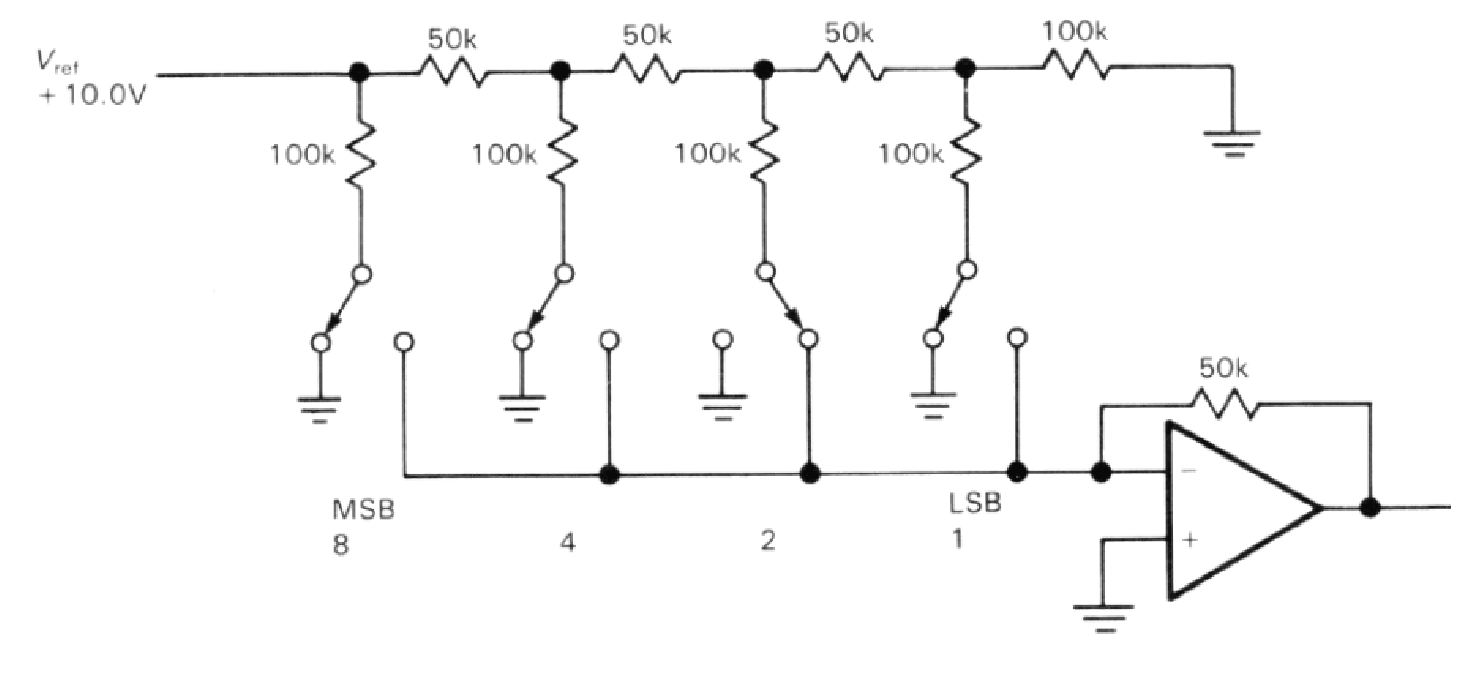
\includegraphics[width=0.75\linewidth]{DAC_R-2R/R-2R_DAC.eps}
\end{center}

\begin{itemize}
\item Solve for the currents through the 2R (100 k$\Omega$) resistors
associated with each bit branch for the binary numbers 1100 and 0011.  (A
switch will be in the GND position when it represents a `0'.)

\begin{center}
\begin{tabular}{|c|c|}\hline
$i_1$ (MSB) & 0.1 mA \\
$i_2$ & 0.05 mA \\
$i_3$ & 0.025 mA \\
$i_4$ (LSB) & 0.0.125 mA \\ \hline
\end{tabular}
\end{center}

\item How do the bit branch currents (1) compare to one another, and (2) change
as a function of the binary digit they represent (0 or 1)?  Does this make
sense?

The currents are $\frac{1}{2}$ the next significant bit's current.  $V_-$ is
always 0 (GND) because of the negative feedback in the op amp and $V_+$ being
tied to GND, so the currents do not change, regardless of the bit states.
$V_{\textrm{out}}$ {\bf does} change as a function of the bit state!

\item What is $V_o$ (the output voltage from the op amp) for the two binary numbers?
\end{itemize}

\begin{center}
1100: $V_{\textrm{out}}$ = -7.5 V \\
0011: $V_{\textrm{out}}$ = -1.875 V
\end{center}
